\documentclass[12pt,x11names,a4paper]{article}
\input{preamble}


\newgeometry{margin=2cm}

\pagestyle{fancy}
\fancyhf{}

\rhead{Nørre Gymnasium\\1.h
}
\cfoot{Side \thepage \hspace{1pt} af \pageref{LastPage}}

%Husk at rette modul og dato!
\lhead{Aflevering 5\\ Matematik A
}
\chead{
}

\begin{document}

%
\includepdf[pages=-]{Forsider/aarsprove_1v.pdf}
\savegeometry{art}

\begin{titlepage}
\newgeometry{margin=0pt}

\begin{minipage}{0.27\textwidth}

\begin{tikzpicture}[overlay]
\fill[top color = NorregGroen!40, bottom color = NorregGroen] (6,10) rectangle (-10,-30);
\end{tikzpicture}
\end{minipage}
\begin{minipage}{0.73\textwidth}
\begin{center}
\phantom{h} \vspace{1cm}\\
\hspace{4cm}

\includegraphics[scale = 1]{Billeder/Norreg.png} \\
\phantom{h} \vspace{5cm}\\
\rule{0.7\textwidth}{0.3mm}\\
\phantom{h}\\
{\fontsize{50}{60}\selectfont Aflevering 5}\\
\phantom{h}\\
\rule{0.7\textwidth}{0.3mm}\\
\Large 2025\\
\Large 1.h MA

\end{center}
\end{minipage}
\end{titlepage}
\loadgeometry{art}

%Udfyld afsnit herunder og lav til egen Latex-fil

%Kopier følgende til overskrift:

%\begin{center}
%\Huge
%Aflevering 1
%\end{center}
%\section*{Opgave 1}
%\stepcounter{section}
\begin{center}
%Opgavesætter er delt i to dele:\\
%Delprøve 1 kun med den centralt udmeldte formelsamling.\\
%Delprøve 2 med alle hjælpemidler.
\end{center}

\section*{Krav til formidling af din besvarelse}

Ved bedømmelse af helhedsindtrykket af besvarelsen af de enkelte opgaver lægges særlig vægt på følgende fire punkter:
\begin{itemize}
\item[$\cdot$] \textbf{Redegørelse og dokumentation for metode} \\
Besvarelsen skal indeholde en redegørelse for den anvendte løsningsstragegi med dokumentation i form af et passende antal mellemregninger \textit{eller} matematiske forklaringer på metoden, når et matematisk værktøjsprogram anvendes.
\item[$\cdot$] \textbf{Figurer, grafer og andre illustrationer} \\
Besvarelsen skal indeholde hensigtsmæssig brug af figurer, grafer og andre illustrationer, og der skal være tydelige henvisninger til brug af disse i den forklarende tekst.
\item[$\cdot$] \textbf{Notation og layout}\\
Besvarelsen skal i overensstemmelse med god matematisk skik opstilles med hensigtsmæssig brug af symbolsprog, og med en redegørelse for den matematiske notation, der indføres og anvendes, og som ikke kan henføres stil standardviden.
\item[$\cdot$] \textbf{Formidling og forklaring}\\
Besvarelsen af rene matematikopgaver skal indeholde en angivelse af givne oplysninger og korte forklaringer knyttet til den anvendte løsningsstrategi beskrevet med brug af almindelig matematisk notation. 

Besvarelsen af opgaver, der omhandler matematiske modeller, skal indeholde en kort præsentation af modellens kontekst, herunder betydning af modellens parametre. De enkelte delspørgsmål skal afsluttes med en præcis konklusion præsenteret i et klart sprog i relation til konteksten.
\end{itemize}

\newpage

\begin{center}
	\LARGE
	Uden hjælpemidler
\end{center}
\begin{opgavetekst}{Opgave 1}
	To mængder $A$ og $B$ er givet ved
	\begin{align*}
		A &= \{1,2,3,4,5\}, \\
		B &= \{2,4,5,6,a,b\}.
	\end{align*}
\end{opgavetekst}
\begin{delopgave}{}{1}
	Bestem $A \cup B$, $A \cap B$ og $A \backslash B$. 
\end{delopgave}
\begin{delopgave}{}{2}
	For to vilkårlige mængder $S$ og $T$ tegn da et Venn-diagram, der illustrerer mængden 
	\begin{align*}
		(S\cup T)\backslash (S\cap T)
	\end{align*}
\end{delopgave}
\begin{delopgave}{}{3}
	Bestem mængden $C$ givet ved
	\begin{align*}
		C = (A\cup B)\backslash (A \cap B).
	\end{align*}
\end{delopgave}
\begin{opgavetekst}{Opgave 2}
	En funktion $f$ er givet ved grafen på Figur \ref{fig:defværd}
	\begin{figure}[H]	
	\centering
	\resizebox{0.45\textwidth}{!}{
	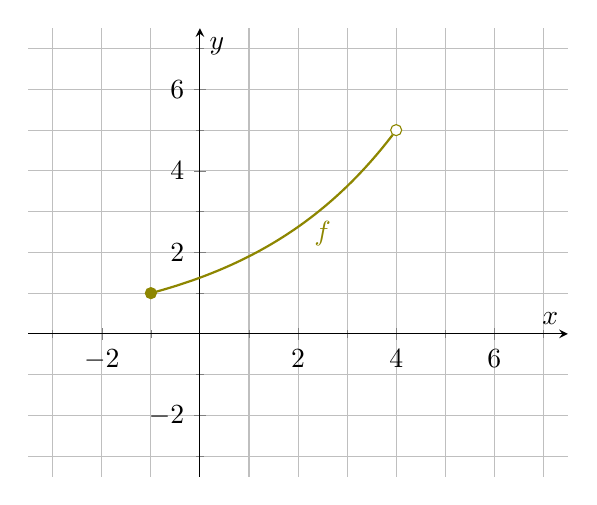
\begin{tikzpicture}
		\begin{axis}
		[axis lines = center, 
		xmin = -3.5, xmax = 7.5,
		ymin = -3.5, ymax = 7.5,
		grid = both,
		xtick = {-4,-2,...,8,10},
		ytick = {-4,-2,...,8,10},
		minor tick num = 1,
		xlabel = $x$, ylabel = $y$
		]
			\addplot[color = olive, thick, domain = -1:4, samples = 200] {1.3797*1.3797^x};	
			\filldraw[color = white](axis cs: 4,5) circle (2pt);
			\draw[color = olive](axis cs: 4,5) circle (2pt);
			\filldraw[color = olive](axis cs: -1,1) circle (2pt);
			\node[color = olive, anchor = north] at (axis cs: 2.5,3) {$f$};
		\end{axis}
	\end{tikzpicture}
	}
	\caption{Graf for funktionen $f$.}
	\label{fig:defværd}
	\end{figure}
	\phantom{h}
\end{opgavetekst}
\begin{delopgave}{}{1}
	Bestem $f(-1)$.
\end{delopgave}
\begin{delopgave}{}{2}
	Bestem definitionsmængden $\textnormal{Dm}(f)$ og værdimængden $\textnormal{Vm}(f)$.
\end{delopgave}

\newpage

\begin{opgavetekst}{Opgave 3}
	En funktion $f: \mathbb{R} \to \mathbb{R}$ er givet ved
	\begin{align*}
		f(x) = 4x-5.
	\end{align*}	 
\end{opgavetekst}

\begin{delopgave}{}{1}
	For mængden $A = \{1,3,5\}$ bestem da billedmængden $f(A)$.
\end{delopgave}
\begin{delopgave}{}{2}
	Bestem urbilledet af $B = \{-9,20,-5\}$ under $f$.
\end{delopgave}

\begin{opgavetekst}{Opgave 4}
	To funktioner $f$ og $g$ er givet ved henholdsvis
	\begin{align*}
		f(x) &= \log_{2}(x), \\
		g(x) &= x^2 - 4x + 4 
	\end{align*}
\end{opgavetekst}
\begin{delopgave}{}{1}
	Bestem $f(g(6))$.
\end{delopgave}

\newpage

\begin{opgavetekst}{Opgave 5}
	Grafen for en stykvist defineret funktion $g$ kan ses af Figur \ref{fig:stykvis}.
	\begin{figure}[H]
		\centering
		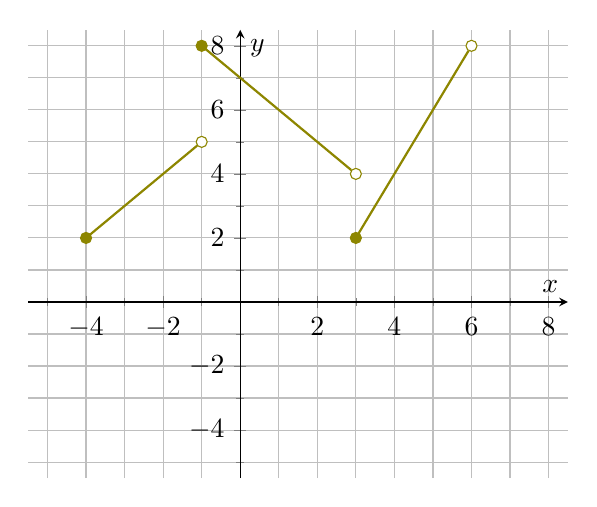
\begin{tikzpicture}
		\begin{axis}
		[
		axis lines = middle, 
		xmin = -5.5, xmax = 8.5,
		ymin = -5.5, ymax = 8.5,
		xtick = {-6,-4,...,8,10},
		ytick = {-6,-4,...,8,10},
		minor tick num = 1,
		xlabel = $x$, ylabel = $y$,	
		grid = both,	
		]
			\addplot[color = olive, thick, domain = -4:-1] {x + 6};
			\addplot[color = olive, thick, domain = -1:3] {-x + 7};
			\addplot[color = olive, thick, domain = 3:6] {2*x - 4};
			\filldraw[color = olive] (axis cs: -4,2) circle (2pt);
			\filldraw[color = white] (axis cs: -1,5) circle (2pt);
			\draw[color = olive] (axis cs: -1,5) circle (2pt);
			\filldraw[color = olive] (axis cs: -1,8) circle (2pt);
			\filldraw[color = white] (axis cs: 3,4) circle (2pt);
			\draw[color = olive] (axis cs: 3,4) circle (2pt);
			\filldraw[color = olive] (axis cs: 3,2) circle (2pt);
			\filldraw[color = white] (axis cs: 6,8) circle (2pt);
			\draw[color = olive] (axis cs: 6,8) circle (2pt);
		\end{axis}
		\end{tikzpicture}
		\caption{Graf for funktionen $g$.}
		\label{fig:stykvis}
	\end{figure}
	\phantom{h}
\end{opgavetekst}
\begin{delopgave}{}{1}
	Opskriv en forskrift for funktionen $g$.
\end{delopgave}
\begin{delopgave}{}{2}
	Bestem løsningerne til ligningen $g(x) = 4$.
\end{delopgave}

\newpage 

\begin{opgavetekst}{Opgave 6}
	Grafen for en funktion $h:[-4,3[ \to [-4,5]$ er givet på Figur \ref{fig:injsur}.
	\begin{figure}[H]
		\centering
		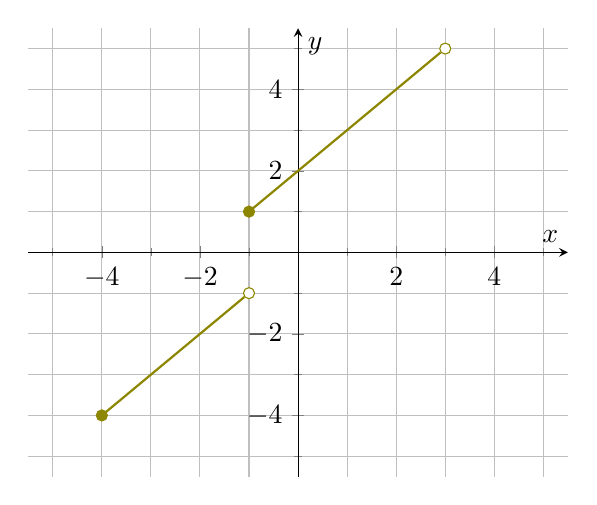
\begin{tikzpicture}
		\begin{axis}
		[
		axis lines = middle, 
		xmin = -5.5, xmax = 5.5,
		ymin = -5.5, ymax = 5.5,
		xtick = {-6,-4,...,8,10},
		ytick = {-6,-4,...,8,10},
		minor tick num = 1,
		xlabel = $x$, ylabel = $y$,	
		grid = both,	
		]
			\addplot[color = olive, thick, domain = -4:-1] {x};
			\addplot[color = olive, thick, domain = -1:3] {x + 2};
			\filldraw[color = olive] (axis cs: -4,-4) circle (2pt);
			\filldraw[color = white] (axis cs: -1,-1) circle (2pt);
			\draw[color = olive] (axis cs: -1,-1) circle (2pt);
			\filldraw[color = olive] (axis cs: -1,1) circle (2pt);
			\filldraw[color = white] (axis cs: 3,5) circle (2pt);
			\draw[color = olive] (axis cs: 3,5) circle (2pt);
		\end{axis}
		\end{tikzpicture}
		\caption{Graf for funktionen $h$.}
		\label{fig:injsur}
	\end{figure}
	\phantom{h}
\end{opgavetekst}
\begin{delopgave}{}{1}
	Afgør, om $h$ er surjektiv, injektiv eller bijektiv. Begrund dit svar.
\end{delopgave}

\begin{opgavetekst}{Opgave 7}
	To funktioner $f$ og $g$ er givet ved henholdsvis
	\begin{align*}
		f(x) &= 5^{3x-7}, \\
		g(x) &= \frac{\log_{5}(x) + 7}{3}.
	\end{align*}
\end{opgavetekst}
\begin{delopgave}{}{1}
	Undersøg, om $f$ og $g$ er hinandens inverse funktioner.
\end{delopgave}	
\begin{delopgave}{}{2}
	Bestem den inverse funktion til $f$ givet ved
	\begin{align*}
		f(x) = 10x - 6.
	\end{align*}
\end{delopgave}


\end{document}




